\documentclass[11pt,a4paper]{article}
\usepackage[utf8]{inputenc} 
\usepackage[T1]{fontenc}
\usepackage[polish]{babel}
\usepackage{amsmath}
\usepackage{graphicx}
\usepackage[a4paper, margin=2.5cm]{geometry}
\usepackage[dvipsnames]{xcolor}
\usepackage{hyperref}
\usepackage{listings}
\usepackage{enumitem}
\usepackage{url}

\graphicspath{ {./images/} }

\hypersetup{
    colorlinks=true,
    linkcolor=blue,
    filecolor=magenta,      
    urlcolor=cyan,
    pdftitle={Raport - Planowanie z wykorzystaniem języka PDDL},
    pdfpagemode=FullScreen,
}

\lstdefinestyle{PDDLstyle}{
    language=Lisp,
    basicstyle=\ttfamily\footnotesize,
    keywordstyle=\color{blue},
    commentstyle=\color{OliveGreen},
    stringstyle=\color{red},
    identifierstyle=\color{black},
    numbers=left,
    numberstyle=\tiny\color{Gray},
    stepnumber=1,
    numbersep=5pt,
    backgroundcolor=\color{Gray!10},
    showspaces=false,
    showstringspaces=false,
    showtabs=false,
    frame=single,
    tabsize=2,
    captionpos=b,
    breaklines=true,
    breakatwhitespace=true,
    title=\lstname,
    escapeinside={\%*}{*)},
    morekeywords={define, domain, problem, :requirements, :types, :predicates, :action, 
                  :parameters, :precondition, :effect, :objects, :init, :goal, 
                  :strips, :typing, :negative-preconditions, :conditional-effects, 
                  :action-costs, :numeric-fluents, :durative-actions, :multi-agent, 
                  increase, assign, decrease, 
                  at, start, end, over, all, when, 
                  and, or, not, 
                  =, <, >, <=, >=, +, -, *, /, 
                  :functions, number, either, agent,
                  location, package, vehicle, city, airport, port, truck, plane, ship,
                  robot, room, ball, arm
                 } 
}
\lstset{style=PDDLstyle}

\title{
    Sztuczna Inteligencja i Inżynieria Wiedzy - Lista nr 3 \\
    \vspace{0.5cm}
    \textbf{Planowanie z wykorzystaniem języka PDDL}
}
\author{Mikołaj Kubś}
\date{\today} 

\begin{document}
\maketitle
\thispagestyle{empty}
\newpage

\tableofcontents
\newpage

\section{Wprowadzenie}
Celem niniejszego raportu jest przedstawienie rozwiązań trzech zadań z zakresu planowania z wykorzystaniem języka PDDL (Planning Domain Definition Language). Lista zadań miała na celu zapoznanie z podstawami języka PDDL, jego rozszerzeniami oraz praktycznym zastosowaniem w modelowaniu i rozwiązywaniu problemów planowania symbolicznego. W ramach zadań zaimplementowano modele dla problemu transportu paczek z rozszerzeniami, sprzątającego robota oraz przeanalizowano gotowy model robota przenoszącego piłki. Do testowania i generowania planów wykorzystano edytor online \url{https://editor.planning.domains}.

\section{Zadanie 1: Transport paczek z rozszerzeniami}
\subsection{Opis problemu i założenia modelu}
Zadanie polegało na zaprojektowaniu, uruchomieniu i analizie planu transportu paczek. Celem było opracowanie modelu logicznego oraz wdrożenie go w formie plików PDDL, uwzględniając następujące rozszerzenia języka PDDL:
\begin{itemize}
  \item \texttt{:strips} - podstawowy model operacji STRIPS,
  \item \texttt{:typing} - typowanie obiektów (np. paczka, lokacja, pojazd),
  \item \texttt{:negative-preconditions} - warunki negatywne,
  \item \texttt{:conditional-effects} - efekty warunkowe (np. dodatkowy koszt dla paczek delikatnych),
  \item \texttt{:numeric-fluents} i \texttt{:action-costs} - koszty działań,
  \item \texttt{:durative-actions} - czas trwania akcji,
  \item Złożona topologia transportu (drogowego, lotniczego oraz wodnego).
  \item Model uwzględniał również możliwość działania wielu pojazdów (aspekt \texttt{:multi-agent} realizowany poprzez definicję wielu obiektów typu pojazd i możliwość ich równoległego (w sensie czasowym) działania w planie).
\end{itemize}
Model został rozwijany iteracyjnie, dodając kolejne funkcjonalności i rozszerzenia, co pozwoliło na stopniowe testowanie i weryfikację poprawności.

\subsection{Definicja domeny (\texttt{domain-task1.pddl})}

\begin{lstlisting}[caption=Domena zadania 1, label=lst:req_task1]
(define (domain package-transport-step6)
  (:requirements :strips :typing :negative-preconditions :action-costs 
                 :durative-actions :conditional-effects)

  (:types
    package
    location
        city airport port - location
    vehicle
        truck plane ship - vehicle
  )

  (:predicates
    (at-pkg ?p - package ?l - location)
    (at-vehicle ?v - vehicle ?l - location)
    (in-pkg ?p - package ?v - vehicle)
    (road-connection ?from - location ?to - location)
    (air-connection ?from - airport ?to - airport)
    (sea-connection ?from - port ?to - port)
    (fragile ?p - package)
  )

  (:functions
    (total-cost) - number
    (travel-distance ?l1 - location ?l2 - location) - number
    (speed ?v - vehicle) - number
    (load-unload-fixed-time) - number
  )

  (:durative-action load-package
    :parameters (?pkg - package ?veh - vehicle ?loc - location)
    :duration (= ?duration (load-unload-fixed-time))
    :condition (and
                 (at start (at-pkg ?pkg ?loc))
                 (at start (at-vehicle ?veh ?loc))
               )
    :effect (and
              (at end (in-pkg ?pkg ?veh))
              (at end (not (at-pkg ?pkg ?loc)))
              ; Conditional costs
              (when (and (at start (fragile ?pkg)))  ; If fragile
                    (at end (increase (total-cost) 15))) ; Total load cost for fragile = 5 (base) + 10 (extra)
              (when (and (at start (not (fragile ?pkg)))) ; If NOT fragile (requires :negative-preconditions also for conditions in 'when')
                    (at end (increase (total-cost) 5)))
            )
  )

  (:durative-action unload-package
    :parameters (?pkg - package ?veh - vehicle ?loc - location)
    :duration (= ?duration (load-unload-fixed-time))
    :condition (and
                 (at start (in-pkg ?pkg ?veh))
                 (at start (at-vehicle ?veh ?loc))
               )
    :effect (and
              (at end (at-pkg ?pkg ?loc))
              (at end (not (in-pkg ?pkg ?veh)))
              (at end (increase (total-cost) 3))
            )
  )

  (:durative-action drive-truck
    :parameters (?tr - truck ?from - location ?to - location)
    :duration (= ?duration (/ (travel-distance ?from ?to) (speed ?tr)))
    :condition (and
                 (at start (at-vehicle ?tr ?from))
                 (over all (road-connection ?from ?to))
               )
    :effect (and
              (at start (not (at-vehicle ?tr ?from)))
              (at end (at-vehicle ?tr ?to))
              (at end (increase (total-cost) 10))
            )
  )

  (:durative-action fly-plane
    :parameters (?pl - plane ?from - airport ?to - airport)
    :duration (= ?duration (/ (travel-distance ?from ?to) (speed ?pl)))
    :condition (and
                 (at start (at-vehicle ?pl ?from))
                 (over all (air-connection ?from ?to))
               )
    :effect (and
              (at start (not (at-vehicle ?pl ?from)))
              (at end (at-vehicle ?pl ?to))
              (at end (increase (total-cost) 100))
            )
  )

  (:durative-action sail-ship
    :parameters (?sh - ship ?from - port ?to - port)
    :duration (= ?duration (/ (travel-distance ?from ?to) (speed ?sh)))
    :condition (and
                 (at start (at-vehicle ?sh ?from))
                 (over all (sea-connection ?from ?to))
               )
    :effect (and
              (at start (not (at-vehicle ?sh ?from)))
              (at end (at-vehicle ?sh ?to))
              (at end (increase (total-cost) 50))
            )
  )
)
\end{lstlisting}

\subsubsection{Typy}
Zdefiniowano hierarchię typów dla lokacji i pojazdów:
\begin{lstlisting}[caption=Typy w domenie Zadania 1, label=lst:types_task1]
(:types
    package
    location
        city airport port - location
    vehicle
        truck plane ship - vehicle
)
\end{lstlisting}

\subsubsection{Predykaty}
Kluczowe predykaty obejmowały:
\begin{lstlisting}[caption=Predykaty w domenie Zadania 1, label=lst:pred_task1]
(at-pkg ?p - package ?l - location)
(at-vehicle ?v - vehicle ?l - location)
(in-pkg ?p - package ?v - vehicle)
(road-connection ?from - location ?to - location)
(air-connection ?from - airport ?to - airport)
(sea-connection ?from - port ?to - port)
(fragile ?p - package)
\end{lstlisting}

\subsubsection{Funkcje (fluenty numeryczne)}
Zdefiniowano następujące fluenty numeryczne:
\begin{lstlisting}[caption=Funkcje w domenie Zadania 1, label=lst:func_task1]
(:functions
    (total-cost) - number
    (travel-distance ?l1 - location ?l2 - location) - number
    (speed ?v - vehicle) - number
    (load-unload-fixed-time) - number
)
\end{lstlisting}

\subsubsection{Akcje (Przykłady)}
Przykładowa akcja \texttt{load-package} z efektem warunkowym oraz akcja \texttt{drive-truck} z czasem trwania:
\begin{lstlisting}[caption=Akcja load-package z efektem warunkowym, label=lst:action_load_task1]
(:durative-action load-package
    :parameters (?pkg - package ?veh - vehicle ?loc - location)
    :duration (= ?duration (load-unload-fixed-time))
    :condition (and
                 (at start (at-pkg ?pkg ?loc))
                 (at start (at-vehicle ?veh ?loc))
               )
    :effect (and
              (at end (in-pkg ?pkg ?veh))
              (at end (not (at-pkg ?pkg ?loc)))
              (when (at start (fragile ?pkg))
                    (at end (increase (total-cost) 10))) 
              (at end (increase (total-cost) 5))
            )
)
\end{lstlisting}
\begin{lstlisting}[caption=Akcja drive-truck z czasem trwania, label=lst:action_drive_task1]
(:durative-action drive-truck
    :parameters (?tr - truck ?from - location ?to - location)
    :duration (= ?duration (/ (travel-distance ?from ?to) (speed ?tr)))
    :condition (and
                 (at start (at-vehicle ?tr ?from))
                 (over all (road-connection ?from ?to))
               )
    :effect (and
              (at start (not (at-vehicle ?tr ?from)))
              (at end (at-vehicle ?tr ?to))
              (at end (increase (total-cost) 10))
            )
)
\end{lstlisting}

\subsection{Definicja problemu (\texttt{problem-task1.pddl})}
\begin{lstlisting}[caption=Definicja problemu zadania 1, label=lst:obj_task1]
(define (problem multi-modal-transport-conditional)
  (:domain package-transport-step6)

  (:objects
    p1 - package
    p2 - package

    london paris newyork - city
    heathrow jfk charlesdegaulle - airport
    dover calais newyork_port - port

    my_truck - truck
    my_plane - plane
    my_ship - ship
    another_truck - truck
  )

  (:init
    (= (total-cost) 0)
    (= (load-unload-fixed-time) 1)

    (= (speed my_truck) 60)
    (= (speed another_truck) 60)
    (= (speed my_plane) 500)
    (= (speed my_ship) 30)

    (= (travel-distance london heathrow) 30) (= (travel-distance heathrow london) 30)
    (= (travel-distance london dover) 80) (= (travel-distance dover london) 80)
    (= (travel-distance paris charlesdegaulle) 20) (= (travel-distance charlesdegaulle paris) 20)
    (= (travel-distance paris calais) 150) (= (travel-distance calais paris) 150)
    (= (travel-distance newyork jfk) 25) (= (travel-distance jfk newyork) 25)
    (= (travel-distance newyork newyork_port) 10) (= (travel-distance newyork_port newyork) 10)
    (= (travel-distance jfk newyork_port) 30) (= (travel-distance newyork_port jfk) 30)
    (= (travel-distance london paris) 350) (= (travel-distance paris london) 350)
    (= (travel-distance heathrow jfk) 3000) (= (travel-distance jfk heathrow) 3000)
    (= (travel-distance heathrow charlesdegaulle) 300) (= (travel-distance charlesdegaulle heathrow) 300)
    (= (travel-distance dover calais) 50) (= (travel-distance calais dover) 50)
    (= (travel-distance calais newyork_port) 3500) (= (travel-distance newyork_port calais) 3500)

    (at-pkg p1 london)
    (fragile p1)
    
    (at-pkg p2 jfk)

    (at-vehicle my_truck london)
    (at-vehicle my_plane heathrow)
    (at-vehicle my_ship dover)
    (at-vehicle another_truck newyork_port) 

    (road-connection london heathrow) (road-connection heathrow london)
    (road-connection london dover) (road-connection dover london)
    (road-connection paris charlesdegaulle) (road-connection charlesdegaulle paris)
    (road-connection paris calais) (road-connection calais paris)
    (road-connection newyork jfk) (road-connection jfk newyork)
    (road-connection newyork newyork_port) (road-connection newyork_port newyork)
    (road-connection jfk newyork_port) (road-connection newyork_port jfk)
    (road-connection london paris) (road-connection paris london)

    (air-connection heathrow jfk) (air-connection jfk heathrow)
    (air-connection heathrow charlesdegaulle) (air-connection charlesdegaulle heathrow)

    (sea-connection dover calais) (sea-connection calais dover)
    (sea-connection calais newyork_port) (sea-connection newyork_port calais)
  )

  (:goal
    (and
        (at-pkg p1 newyork)
        (at-pkg p2 calais)
    )
  )

  (:metric minimize (total-cost)) 
)
\end{lstlisting}

\subsubsection{Stan początkowy}
W stanie początkowym zdefiniowano wartości dla fluentów numerycznych (koszt, czasy, prędkości, dystanse), położenie paczek i pojazdów, status paczki pierwszej jako delikatna oraz połączenia między lokacjami.
\begin{lstlisting}[caption=Fragment stanu początkowego w problemie Zadania 1, label=lst:init_task1]
(:init
    (= (total-cost) 0)
    (= (load-unload-fixed-time) 1)
    (= (speed my_truck) 60)
    (= (speed my_plane) 500)
    (= (travel-distance london heathrow) 30)
    (at-pkg p1 london)
    (fragile p1)
    (at-pkg p2 jfk)
    (at-vehicle my_truck london)
    (at-vehicle my_plane heathrow)
    (road-connection london heathrow) 
    (air-connection heathrow jfk)
)
\end{lstlisting}

\subsubsection{Cel i metryka}
Celem było dostarczenie paczki z Londynu \texttt{p1} do Nowego Jorku i paczki \texttt{p2} z JFK do Calais, minimalizując całkowity koszt.
\begin{lstlisting}[caption=Cel i metryka w problemie Zadania 1, label=lst:goal_task1]
(:goal
  (and
      (at-pkg p1 newyork)
      (at-pkg p2 calais)
  )
)
(:metric minimize (total-cost)) 
\end{lstlisting}

\subsection{Wygenerowany plan}
Testy przeprowadzono w edytorze online \url{https://editor.planning.domains} z użyciem solvera \texttt{Temporal Fast Downward planning system}. Poniżej znajduje się wygenerowany plan.
\begin{lstlisting}[caption=Fragment wygenerowanego planu dla Zadania 1, label=lst:plan_task1, basicstyle=\ttfamily\scriptsize, breaklines=true]
0.00100000: (drive-truck another_truck newyork_port newyork) [0.16666700]
0.00100000: (load-package p1 my_truck london) [1.00000000]
0.01100000: (drive-truck my_truck london heathrow) [0.50000000]
1.01100000: (unload-package p1 my_truck heathrow) [1.00000000]
0.17766700: (drive-truck another_truck newyork jfk) [0.41666700]
0.60433400: (drive-truck another_truck jfk newyork) [0.41666700]
2.02100000: (load-package p1 my_plane heathrow) [1.00000000]
1.03100100: (drive-truck another_truck newyork jfk) [0.41666700]
2.03100000: (fly-plane my_plane heathrow jfk) [6.00000000]
1.45766800: (drive-truck another_truck jfk newyork) [0.41666700]
1.88433500: (drive-truck another_truck newyork jfk) [0.41666700]
2.31100200: (drive-truck another_truck jfk newyork) [0.41666700]
2.73766900: (drive-truck another_truck newyork jfk) [0.41666700]
3.16433600: (drive-truck another_truck jfk newyork) [0.41666700]
3.59100300: (drive-truck another_truck newyork jfk) [0.41666700]
4.01767000: (drive-truck another_truck jfk newyork) [0.41666700]
4.44433700: (drive-truck another_truck newyork jfk) [0.41666700]
4.87100400: (drive-truck another_truck jfk newyork) [0.41666700]
5.29767100: (drive-truck another_truck newyork jfk) [0.41666700]
5.72433800: (drive-truck another_truck jfk newyork) [0.41666700]
6.15100500: (drive-truck another_truck newyork jfk) [0.41666700]
6.57767200: (drive-truck another_truck jfk newyork) [0.41666700]
8.04100000: (unload-package p1 my_plane jfk) [1.00000000]
7.00433900: (drive-truck another_truck newyork jfk) [0.41666700]
9.05200000: (load-package p1 another_truck jfk) [1.00000000]
9.06200000: (drive-truck another_truck jfk newyork) [0.41666700]
10.06200000: (unload-package p1 another_truck newyork) [1.00000000]
8.04200000: (load-package p2 my_plane jfk) [1.00000000]
1.02100000: (drive-truck my_truck heathrow london) [0.50000000]
8.05200000: (fly-plane my_plane jfk heathrow) [6.00000000]
0.00100000: (sail-ship my_ship dover calais) [1.66667000]
1.53100000: (drive-truck my_truck london dover) [1.33333000]
1.67767000: (sail-ship my_ship calais dover) [1.66667000]
2.87433000: (drive-truck my_truck dover london) [1.33333000]
4.21766000: (drive-truck my_truck london dover) [1.33333000]
3.35434000: (sail-ship my_ship dover calais) [1.66667000]
5.56099000: (drive-truck my_truck dover london) [1.33333000]
14.06200000: (unload-package p2 my_plane heathrow) [1.00000000]
6.90432000: (drive-truck my_truck london heathrow) [0.50000000]
15.07200000: (load-package p2 my_truck heathrow) [1.00000000]
15.08200000: (drive-truck my_truck heathrow london) [0.50000000]
15.59200000: (drive-truck my_truck london dover) [1.33333000]
5.03101000: (sail-ship my_ship calais dover) [1.66667000]
16.93533000: (unload-package p2 my_truck dover) [1.00000000]
17.94533000: (load-package p2 my_ship dover) [1.00000000]
17.95533000: (sail-ship my_ship dover calais) [1.66667000]
19.63200000: (unload-package p2 my_ship calais) [1.00000000]
\end{lstlisting}

\subsection{Analiza planu i eksperymenty}
\begin{itemize}
  \item \textbf{Logika planu:} Planner poprawnie wybrał trasę multimodalną (ciężarówka do lotniska, samolot, ciężarówka z lotniska) w celu dostarczenia paczki.
  \item \textbf{Koszty i czas trwania:} Wprowadzenie kosztów pozwoliło na optymalizację planu pod kątem minimalizacji wydatków. Akcje czasowe z dynamicznie obliczanym czasem trwania (na podstawie dystansu i prędkości) umożliwiły realistyczne modelowanie operacji logistycznych i obliczenie całkowitego czasu realizacji (makespan).
  \item \textbf{Efekty warunkowe:} Dodatkowy koszt załadunku dla paczki oznaczonej jako delikatna (\texttt{(fragile p1)}) został poprawnie naliczony, co zwiększyło całkowity koszt planu (z 144 do 174 dla ścieżki paczki \texttt{p1}) bez zmiany samej trasy, gdyż trasa lotnicza nadal była optymalna kosztowo.
  \item \textbf{Wybór solvera:} Kluczowe okazało się użycie solvera \texttt{Temporal Fast Downward planning system}, który poprawnie obsługiwał akcje czasowe i inne zaawansowane rozszerzenia PDDL 2.1. Wcześniejsze próby z solverami nieobsługującymi akcji czasowych prowadziły do błędów parsowania.
  \item \textbf{Zachowanie "niekrytycznych" agentów:} Zaobserwowano, że pojazd \texttt{another\_truck}, który nie był na ścieżce krytycznej transportu paczki \texttt{p1} (ale był potrzebny na końcu), wykonywał w planie serię ruchów "jałowych". Jest to cecha planowania automatycznego, gdzie planner może wypełniać czas akcjami, które nie pogarszają metryki optymalizacyjnej i nie blokują osiągnięcia celu.
  \item \textbf{Iteracyjny rozwój i debugowanie:} Podczas implementacji napotkano różne błędy parsowania (np. \texttt{KeyError}, \texttt{AttributeError}, \texttt{AssertionError}), które wynikały z subtelnych błędów składniowych lub niekompatybilności z oczekiwaniami konkretnego parsera/planisty (np. kolejność efektów w akcji, konieczność jawnego określenia czasu dla warunków w efektach warunkowych w akcjach czasowych). Rozwiązywanie tych problemów było cennym doświadczeniem w praktycznym stosowaniu PDDL.
\end{itemize}

\section{Zadanie 2: Sprzątający robot}
\subsection{Opis Problemu}
Zadanie polegało na stworzeniu modelu PDDL dla robota, który ma odwiedzić wszystkie zdefiniowane pokoje i posprzątać je. Robot może przemieszczać się między połączonymi pokojami i wykonywać akcję sprzątania w pokoju, w którym aktualnie się znajduje.

\subsection{Definicja domeny (\texttt{domain-task2.pddl})}
\begin{lstlisting}[language=Lisp, style=PDDLstyle]
(define (domain cleaning-robot-world)
  (:requirements :strips :typing :negative-preconditions)

  (:types
    robot
    room
  )

  (:predicates
    (at ?r - robot ?p - room)
    (is_dirty ?p - room)
    (is_clean ?p - room)
    (connected ?p1 - room ?p2 - room)
  )

  (:action move
    :parameters (?r - robot ?from_room - room ?to_room - room)
    :precondition (and
                    (at ?r ?from_room)   
                    (connected ?from_room ?to_room) 
                  )
    :effect (and
              (not (at ?r ?from_room))
              (at ?r ?to_room)       
            )
  )

  (:action clean_current_room 
    :parameters (?r - robot ?p_to_clean - room)
    :precondition (and
                    (at ?r ?p_to_clean) 
                    (is_dirty ?p_to_clean)
                  )
    :effect (and
              (not (is_dirty ?p_to_clean)) 
              (is_clean ?p_to_clean)    
            )
  )
)
\end{lstlisting}

\begin{itemize}
  \item \textbf{Wymagania:} \texttt{:strips, :typing, :negative-preconditions}.
  \item \textbf{Typy:} \texttt{robot, room}.
  \item \textbf{Predykaty:} \texttt{(at ?r - robot ?p - room)}, \texttt{(is\_dirty ?p - room)}, \texttt{(is\_clean ?p - room)}, \texttt{(connected ?p1 - room ?p2 - room)}.
  \item \textbf{Akcje:}
        \begin{itemize}
          \item \texttt{move (?r - robot ?from\_room - room ?to\_room - room)}: Przesuwa robota z \texttt{?from\_room} do \texttt{?to\_room}, jeśli są połączone i robot jest w \texttt{?from\_room}.
          \item \texttt{clean\_current\_room (?r - robot ?p\_to\_clean - room)}: Sprząta pokój \texttt{?p\_to\_clean}, jeśli robot jest w tym pokoju i pokój jest brudny. Efektem jest zmiana statusu pokoju z \texttt{is\_dirty} na \texttt{is\_clean}.
        \end{itemize}
\end{itemize}

\subsection{Definicja problemu (\texttt{problem-task2.pddl})}
\begin{lstlisting}[language=Lisp, style=PDDLstyle]
(define (problem clean-all-rooms-task) 
  (:domain cleaning-robot-world)

  (:objects
    r1 - robot
    p1 p2 p3 - room
  )

  (:init
    (at r1 p1)
    (is_dirty p1)
    (is_dirty p2)
    (is_dirty p3)

    (connected p1 p2) (connected p2 p1)
    (connected p2 p3) (connected p3 p2)
  )

  (:goal
    (and
        (is_clean p1)
        (is_clean p2)
        (is_clean p3)
    )
  )
)
\end{lstlisting}
\begin{itemize}
  \item \textbf{Obiekty:} \texttt{r1 - robot}, \texttt{p1, p2, p3 - room}.
  \item \textbf{Stan początkowy:} Robot w \texttt{p1}, wszystkie pokoje brudne. Zdefiniowano połączenia umożliwiające robotowi dotarcie do wszystkich pokoi (np. \texttt{(connected p1 p2)}, \texttt{(connected p2 p1)}, \texttt{(connected p2 p3)}, \texttt{(connected p3 p2)}).
  \item \textbf{Cel:} Wszystkie pokoje są czyste: \texttt{(and (is\_clean p1) (is\_clean p2) (is\_clean p3))}.
\end{itemize}

\subsection{Wygenerowany plan}
Do rozwiązania użyto solvera \texttt{BFWS -- FF-parser version}. Wygenerowany plan:
\begin{lstlisting}[caption=Wygenerowany plan dla Zadania 2, label=lst:plan_task2]
(clean_current_room r1 p1)
(move r1 p1 p2)
(clean_current_room r1 p2)
(move r1 p2 p1)
(move r1 p1 p3)
(clean_current_room r1 p3)
\end{lstlisting}

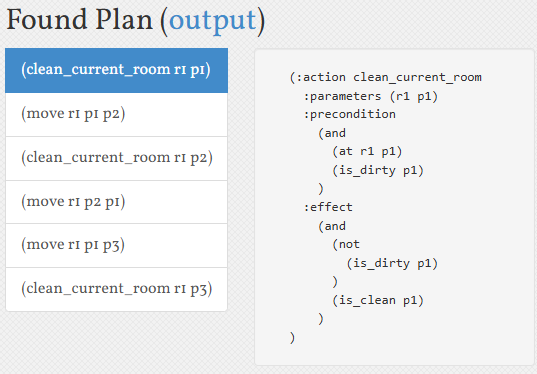
\includegraphics{2}

\subsection{Analiza planu}
Planner poprawnie wygenerował sekwencję akcji, która prowadzi do posprzątania wszystkich pokoi. Kluczowe było zdefiniowanie odpowiedniej topologii połączeń między pokojami, aby umożliwić robotowi dotarcie do każdego z nich. Jeśli początkowo połączenia były zdefiniowane tylko w jedną stronę lub nie tworzyły spójnego grafu, planner nie był w stanie znaleźć rozwiązania. Plan jest sekwencyjny i logiczny.

\section{Zadanie 3: Robot z dwoma ramionami przenoszący piłki}
\subsection{Opis problemu}
Zadanie polegało na analizie dostarczonego modelu PDDL dla robota z dwoma ramionami, który ma przenieść cztery piłki z jednego pokoju do drugiego. Robot może poruszać się między pokojami oraz podnosić i odkładać piłki każdym z ramion.

\subsection{Analiza dostarczonych plików PDDL}
Przeanalizowano dostarczone pliki \texttt{domain-task3.pddl} i \texttt{problem-task3.pddl}.
\begin{itemize}
  \item \textbf{Domena:} Definiuje typy (\texttt{robot, room, ball, arm}) oraz predykaty opisujące stan świata (\texttt{at}, \texttt{inroom}, \texttt{holding}, \texttt{arm-empty}). Akcje to \texttt{move}, \texttt{pick-up} i \texttt{put-down}. Model jest klasycznym przykładem problemu STRIPS.
  \item \textbf{Problem:} Definiuje dwa pokoje, jednego robota (\texttt{robot1}), cztery piłki i dwa ramiona. Stan początkowy umieszcza robota i wszystkie piłki w \texttt{room1}, a ramiona są puste. Celem jest przeniesienie wszystkich piłek do \texttt{room2}.
\end{itemize}
W dostarczonym kodzie problemu poprawiono nazwę obiektu robota na \texttt{robot1} dla spójności.

\subsection{Wygenerowany plan}
Do rozwiązania użyto solvera \texttt{LAMA-first: satisficing planner}. Wygenerowany plan:
\begin{lstlisting}[caption=Wygenerowany plan dla Zadania 3, label=lst:plan_task3]
(pick-up robot1 arm1 ball1 room1)
(pick-up robot1 arm2 ball2 room1)
(move robot1 room1 room2)
(put-down robot1 arm1 ball1 room2)
(put-down robot1 arm2 ball2 room2)
(move robot1 room2 room1)
(pick-up robot1 arm1 ball3 room1)
(pick-up robot1 arm2 ball4 room1)
(move robot1 room1 room2)
(put-down robot1 arm1 ball3 room2)
(put-down robot1 arm2 ball4 room2)
\end{lstlisting}

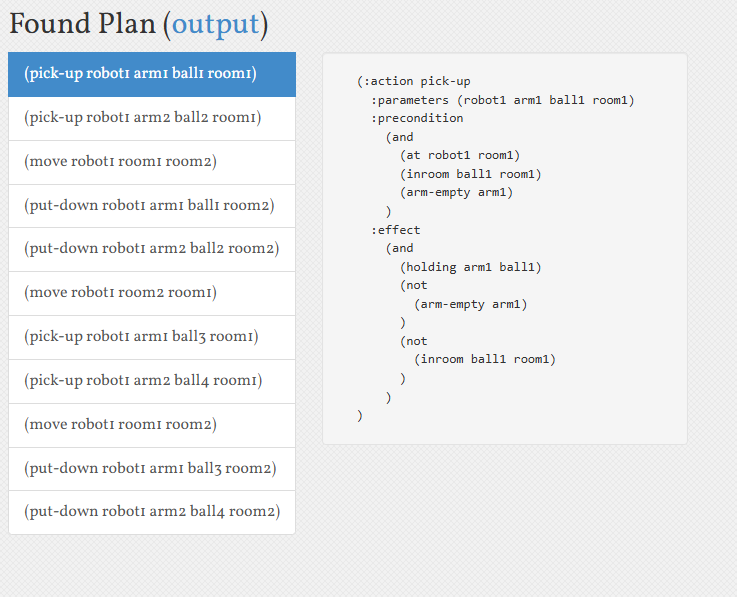
\includegraphics{3}

\subsection{Analiza planu}
\begin{itemize}
  \item \textbf{Wykorzystanie ramion:} Planner efektywnie wykorzystał oba ramiona robota, podnosząc dwie piłki przed każdym przejściem do drugiego pokoju. Skraca to liczbę koniecznych podróży między pokojami.
  \item \textbf{Optymalność:} Wygenerowany plan wydaje się optymalny pod względem liczby kroków dla domyślnych ustawień planera STRIPS, który dąży do minimalizacji liczby akcji. Robot wykonuje minimalną liczbę podróży (dwie do pokoju docelowego i jedna z powrotem).
  \item \textbf{Logika:} Sekwencja akcji jest logiczna i bezpośrednio prowadzi do osiągnięcia celu. Robot najpierw zbiera maksymalną liczbę piłek, jaką może unieść (dwie), transportuje je, odkłada, a następnie wraca po kolejne.
\end{itemize}

\section{Wnioski}
Realizacja zadań z listy nr 3 pozwoliła na praktyczne zapoznanie się z językiem PDDL i jego zastosowaniami w automatycznym planowaniu.
\begin{itemize}
  \item \textbf{Zalety PDDL:} Język jest wysoce ekspresywny, pozwala na deklaratywne opisanie problemu, oddzielając definicję świata od strategii jego rozwiązania. Rozszerzenia PDDL (czas, koszty, efekty warunkowe) umożliwiają modelowanie złożonych, realistycznych problemów.
  \item \textbf{Wady/Wyzwania PDDL:} Składnia, mimo że logiczna, wymaga precyzji i uwagi na detale. Debugowanie może być czasochłonne, a komunikaty błędów od planerów nie zawsze są jednoznaczne. Wybór odpowiedniego planera i jego konfiguracji jest kluczowy dla skutecznego rozwiązania problemu, zwłaszcza przy użyciu zaawansowanych rozszerzeń.
  \item \textbf{Napotkane trudności:} Główne trudności dotyczyły poprawnej składni zaawansowanych funkcji PDDL (np. efekty warunkowe w akcjach czasowych) i zapewnienia kompatybilności modelu z możliwościami wybranego solvera w edytorze online. Iteracyjne podejście do budowy modelu oraz analiza komunikatów błędów pozwoliły na przezwyciężenie tych problemów.
\end{itemize}
Praca z PDDL była cennym doświadczeniem, rozwijającym umiejętności modelowania logicznego i abstrakcyjnego myślenia o problemach.

\end{document}